\chapter{Imagini ale Proiectului Finalizat}

\begin{figure}[h!]
  \centering

  % Rândul 1
  \begin{subfigure}[b]{0.3\textwidth} % 1-a imagine
      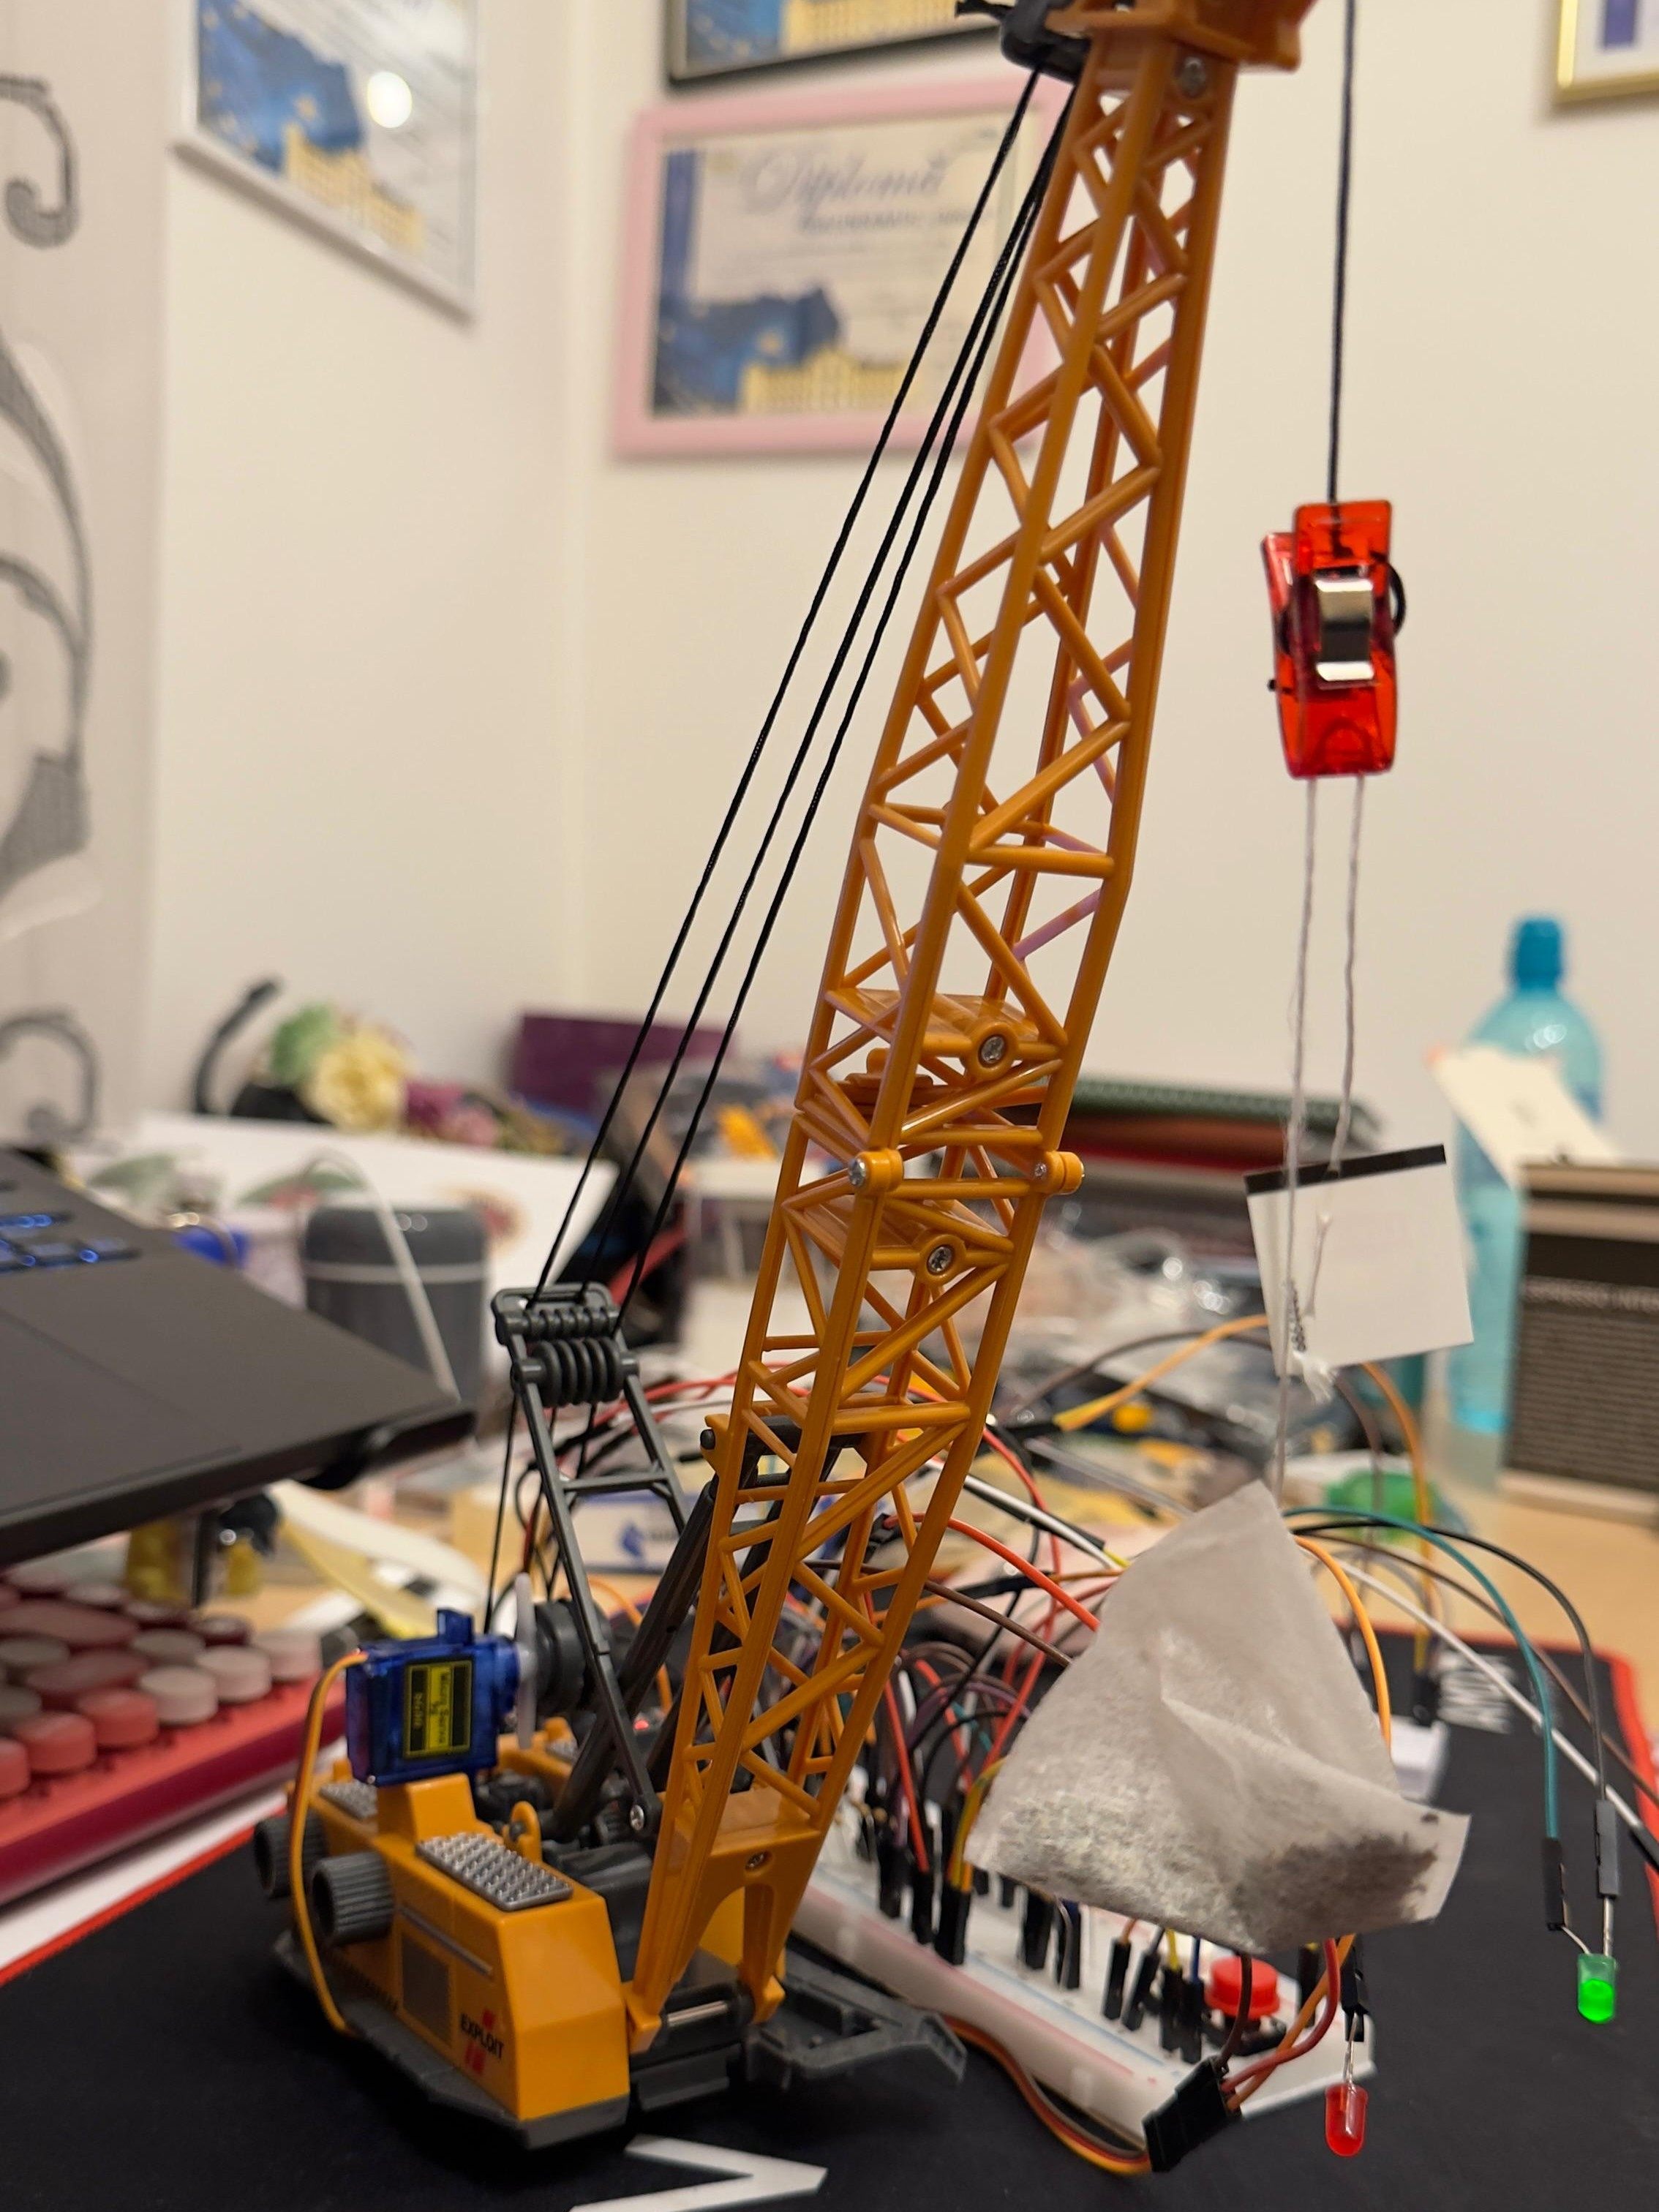
\includegraphics[width=\textwidth]{figures/1.jpg}
      \caption{Macara de jucărie}
  \end{subfigure}
  \hfill
  \begin{subfigure}[b]{0.3\textwidth} % 2-a imagine
      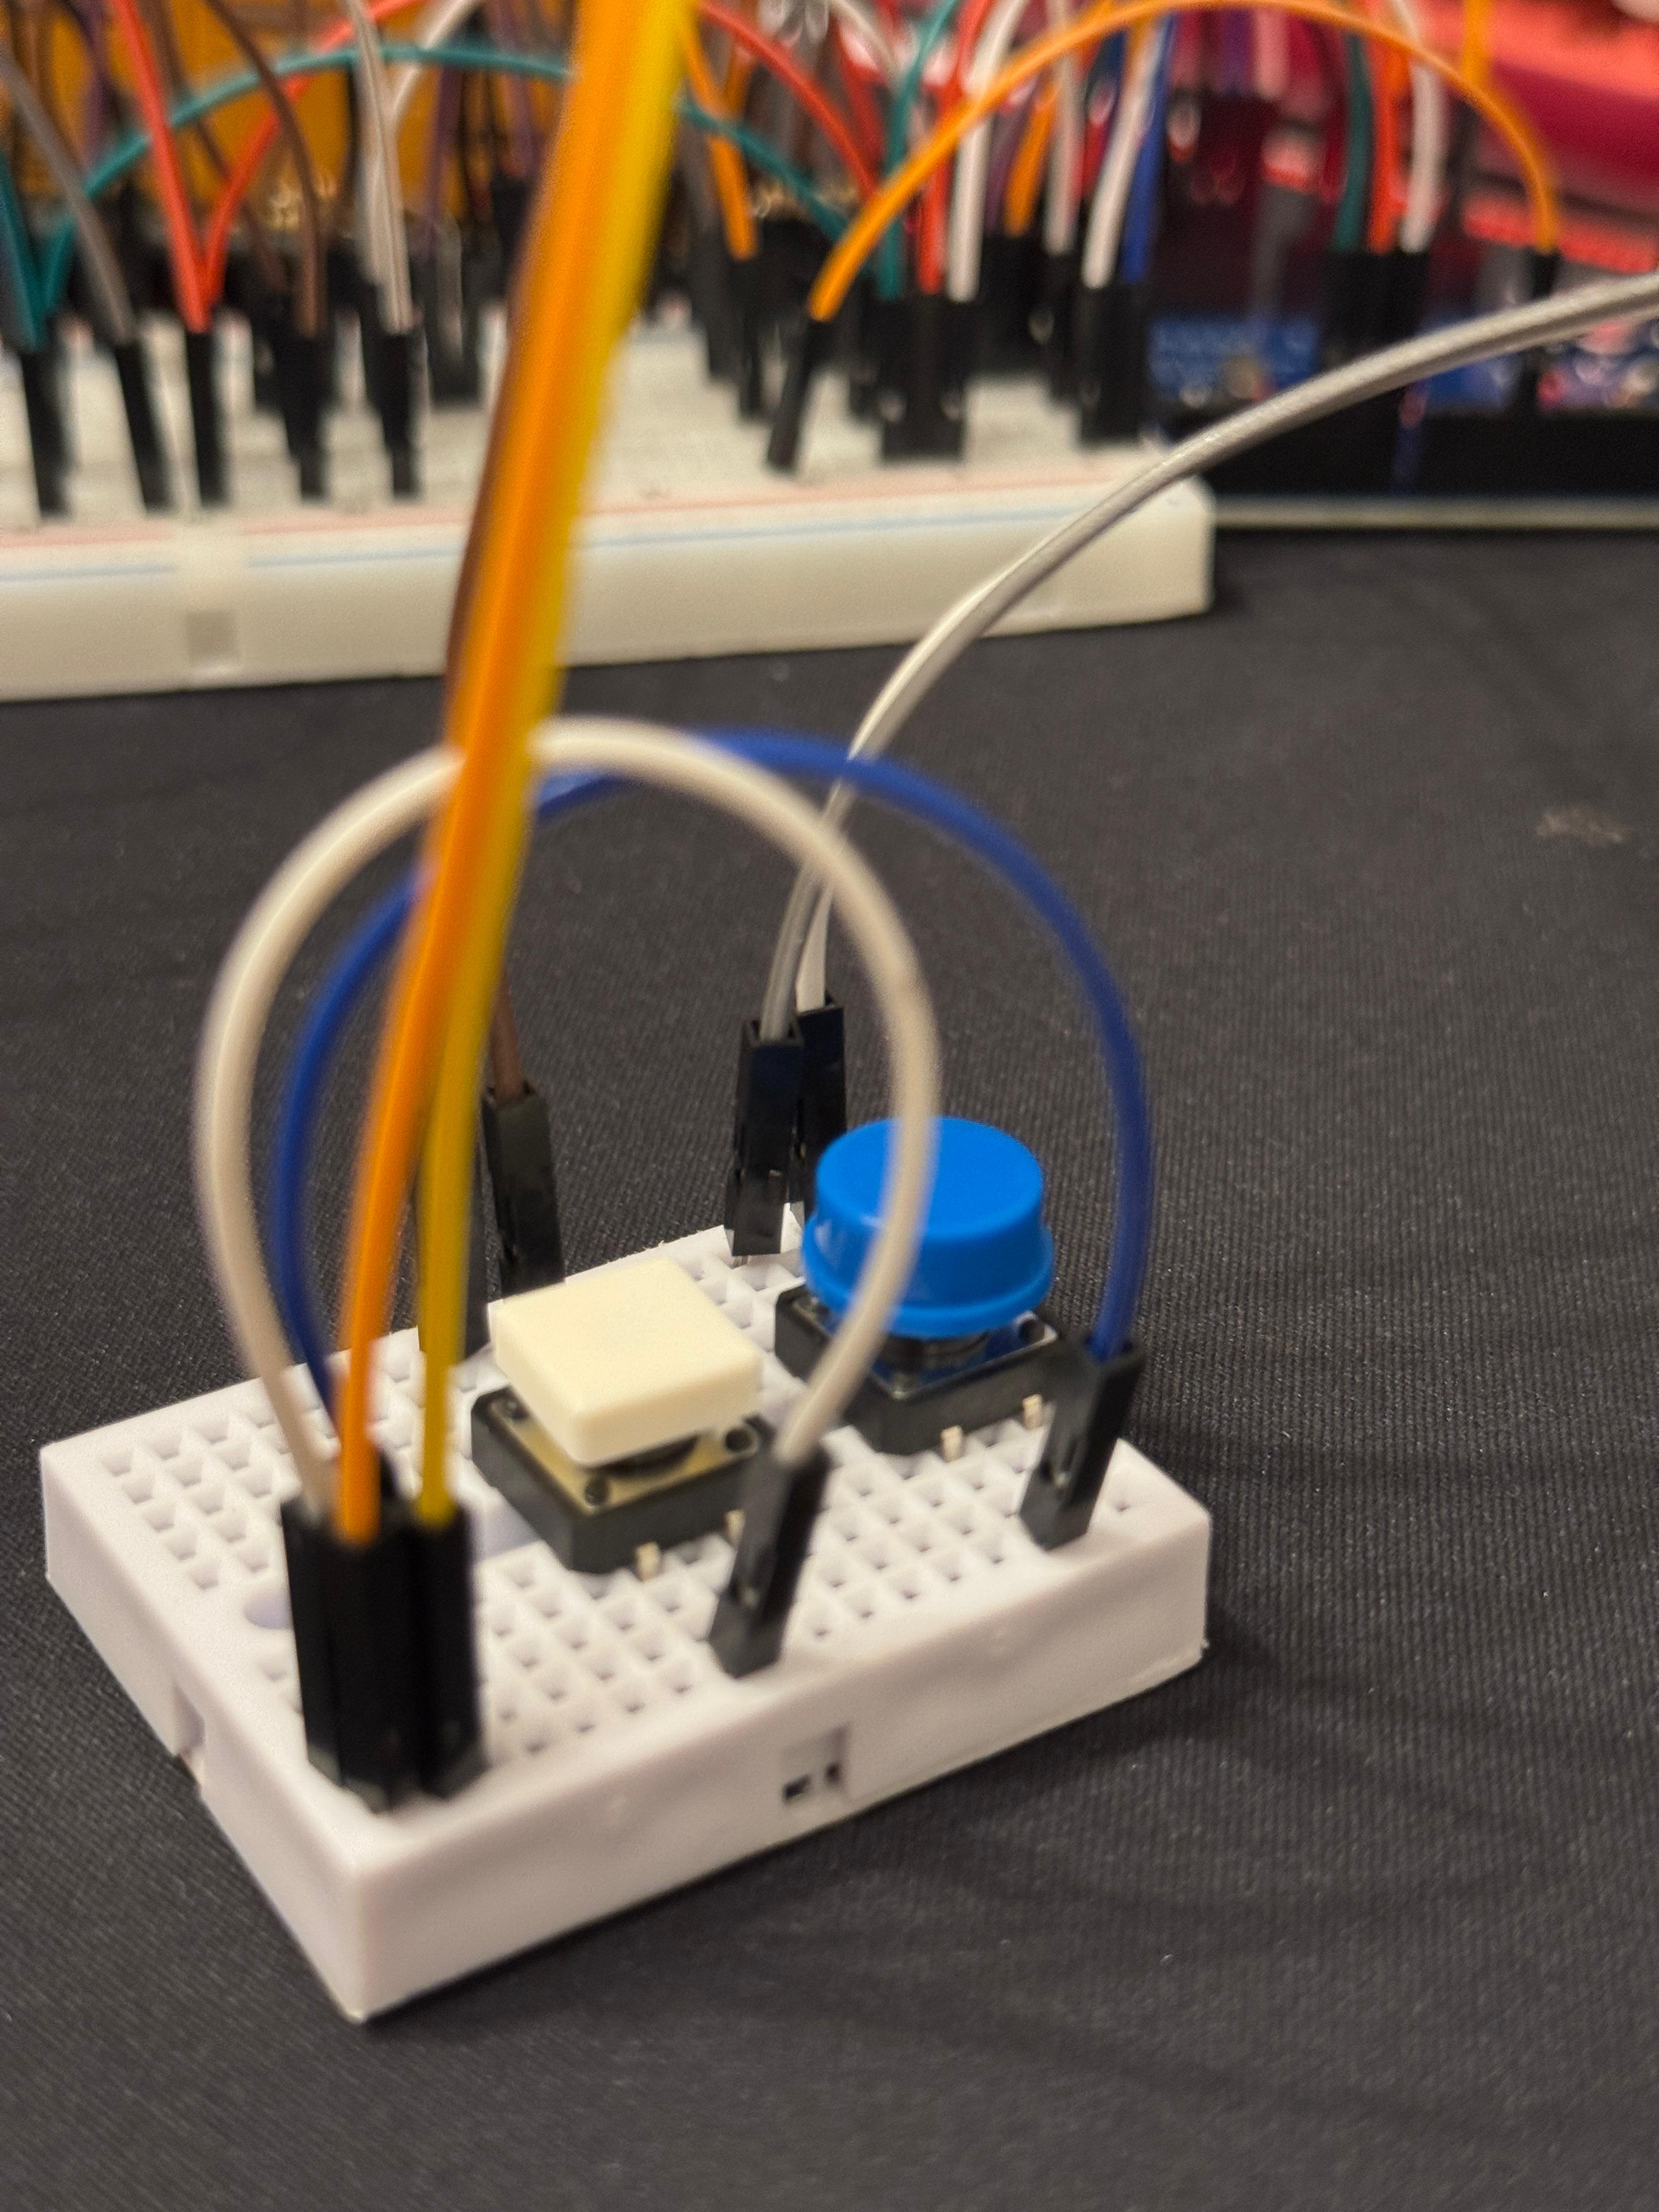
\includegraphics[width=\textwidth]{figures/2.jpg}
      \caption{Butoane Count și Start}
  \end{subfigure}
  \hfill
  \begin{subfigure}[b]{0.3\textwidth} % 3-a imagine
      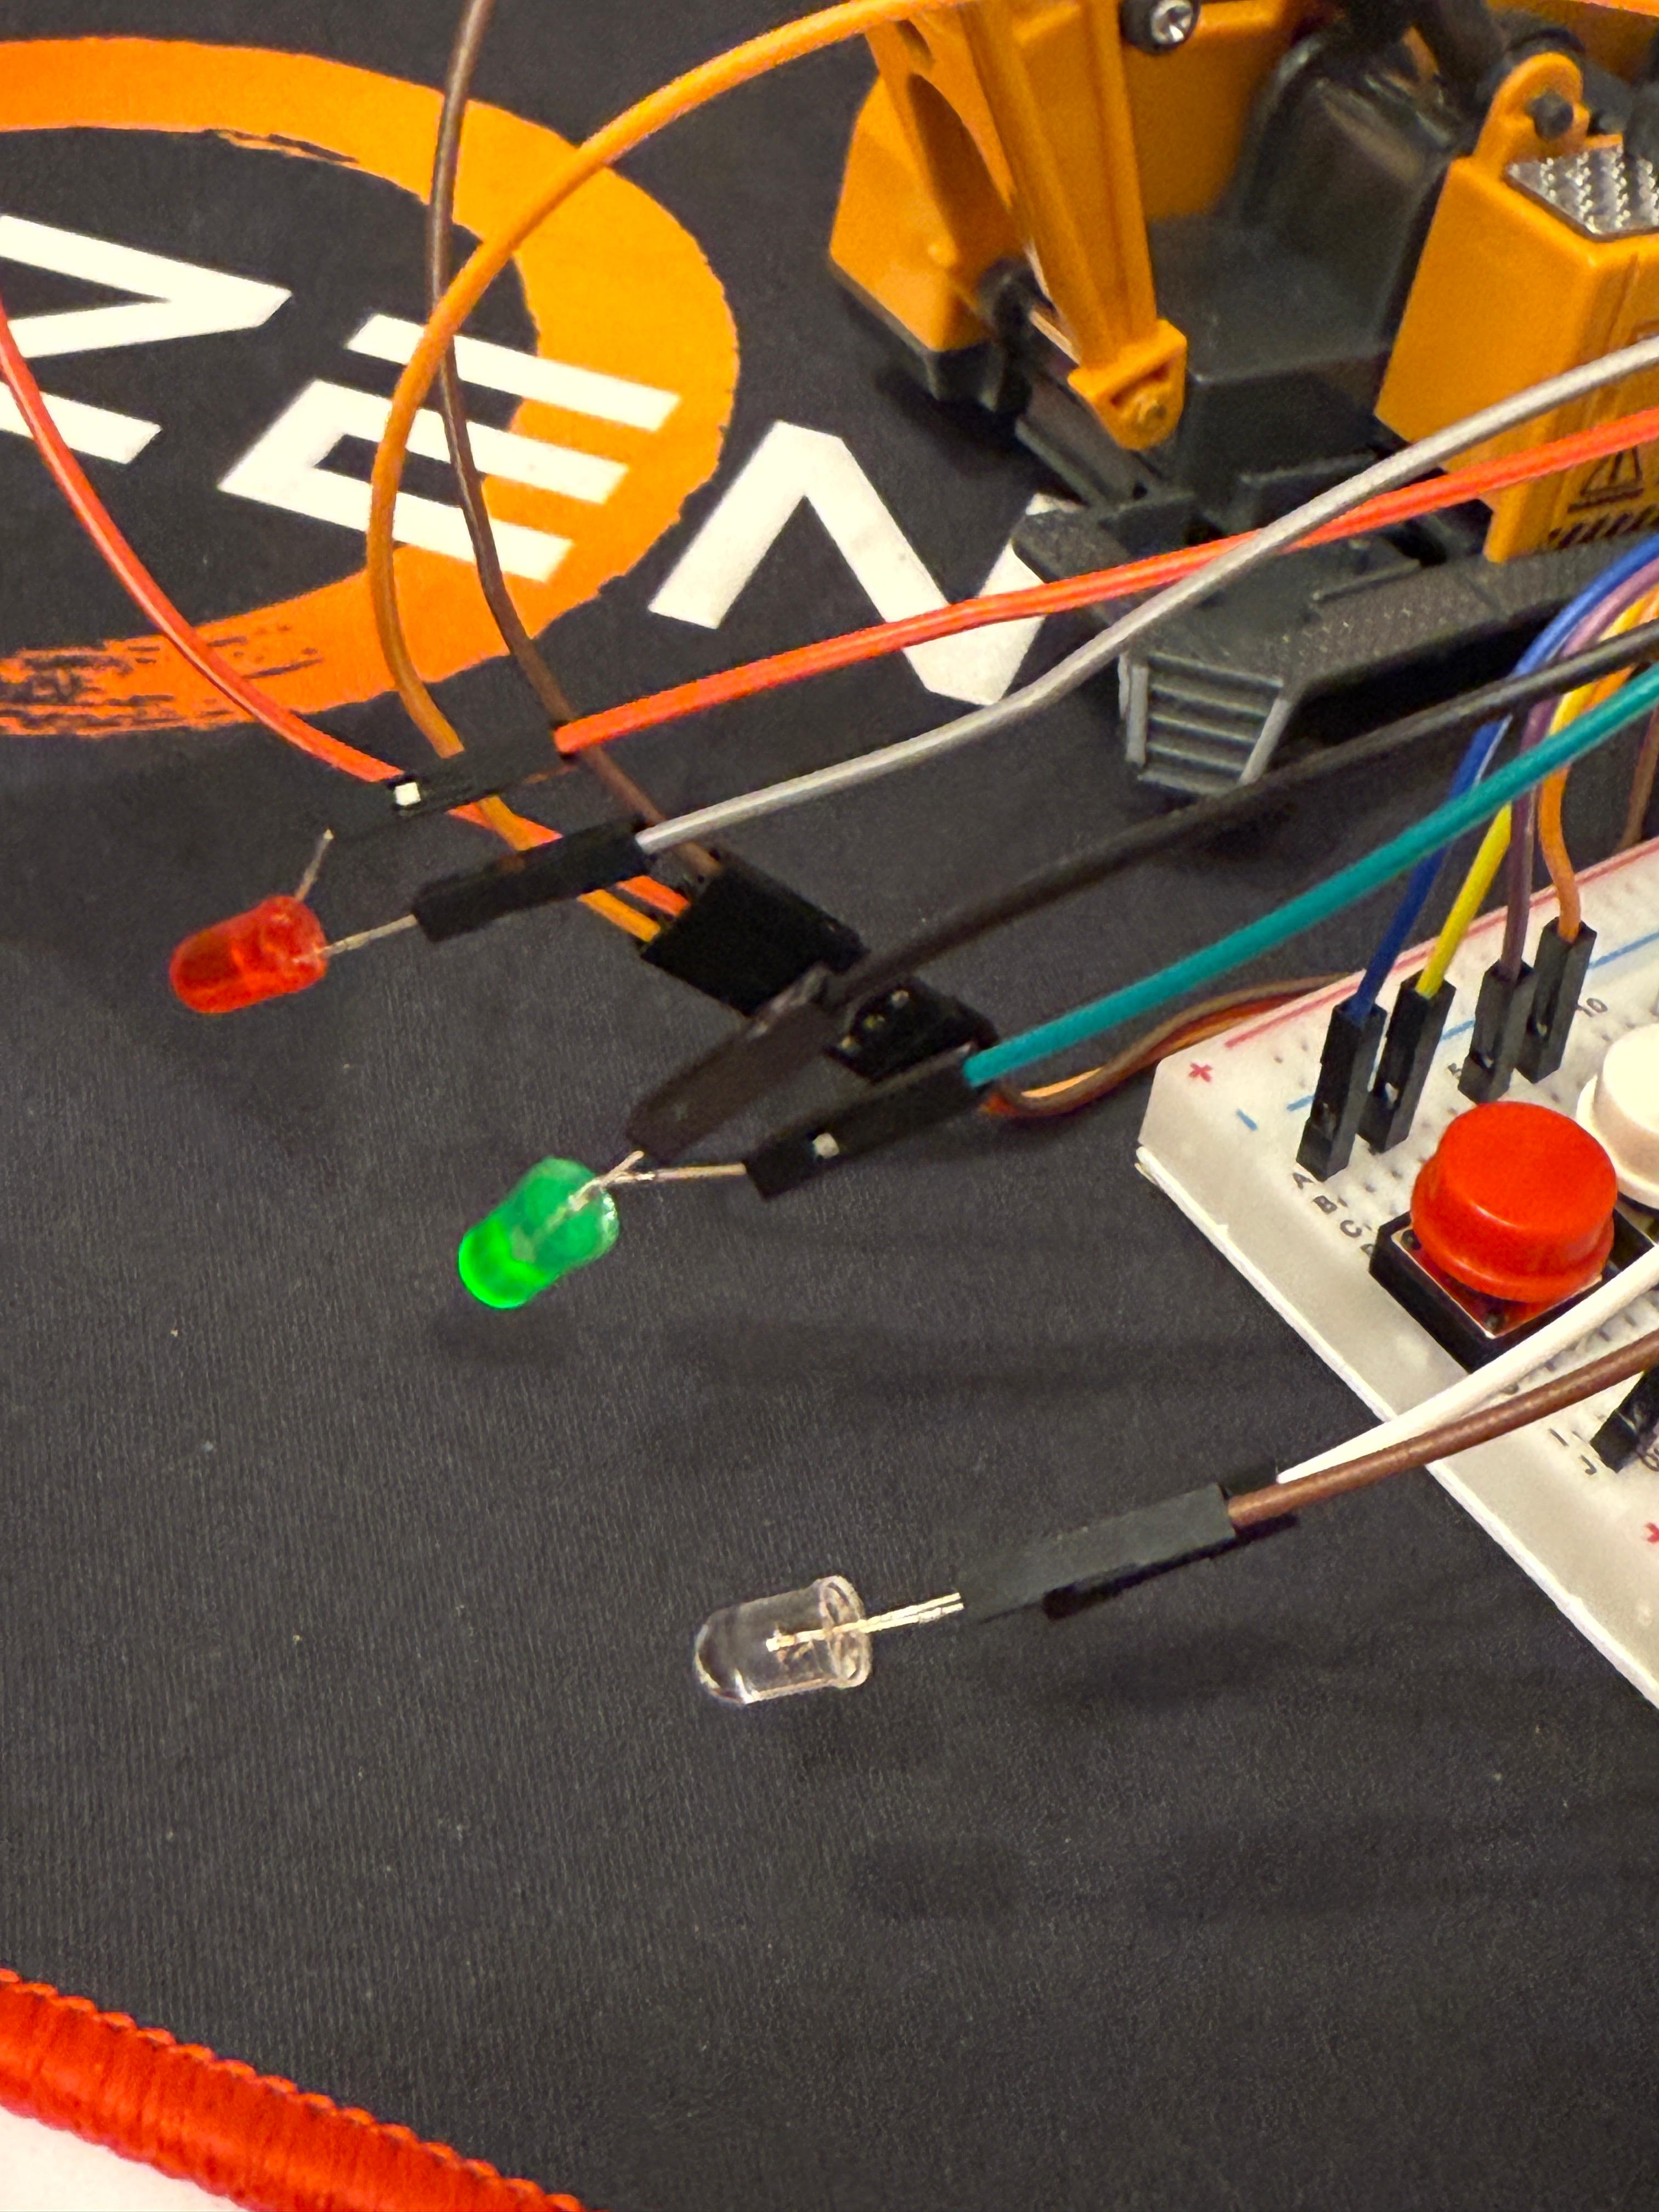
\includegraphics[width=\textwidth]{figures/3.jpg}
      \caption{LED-uri}
  \end{subfigure}

  % Rândul 2
  \begin{subfigure}[b]{0.3\textwidth} % 4-a imagine
      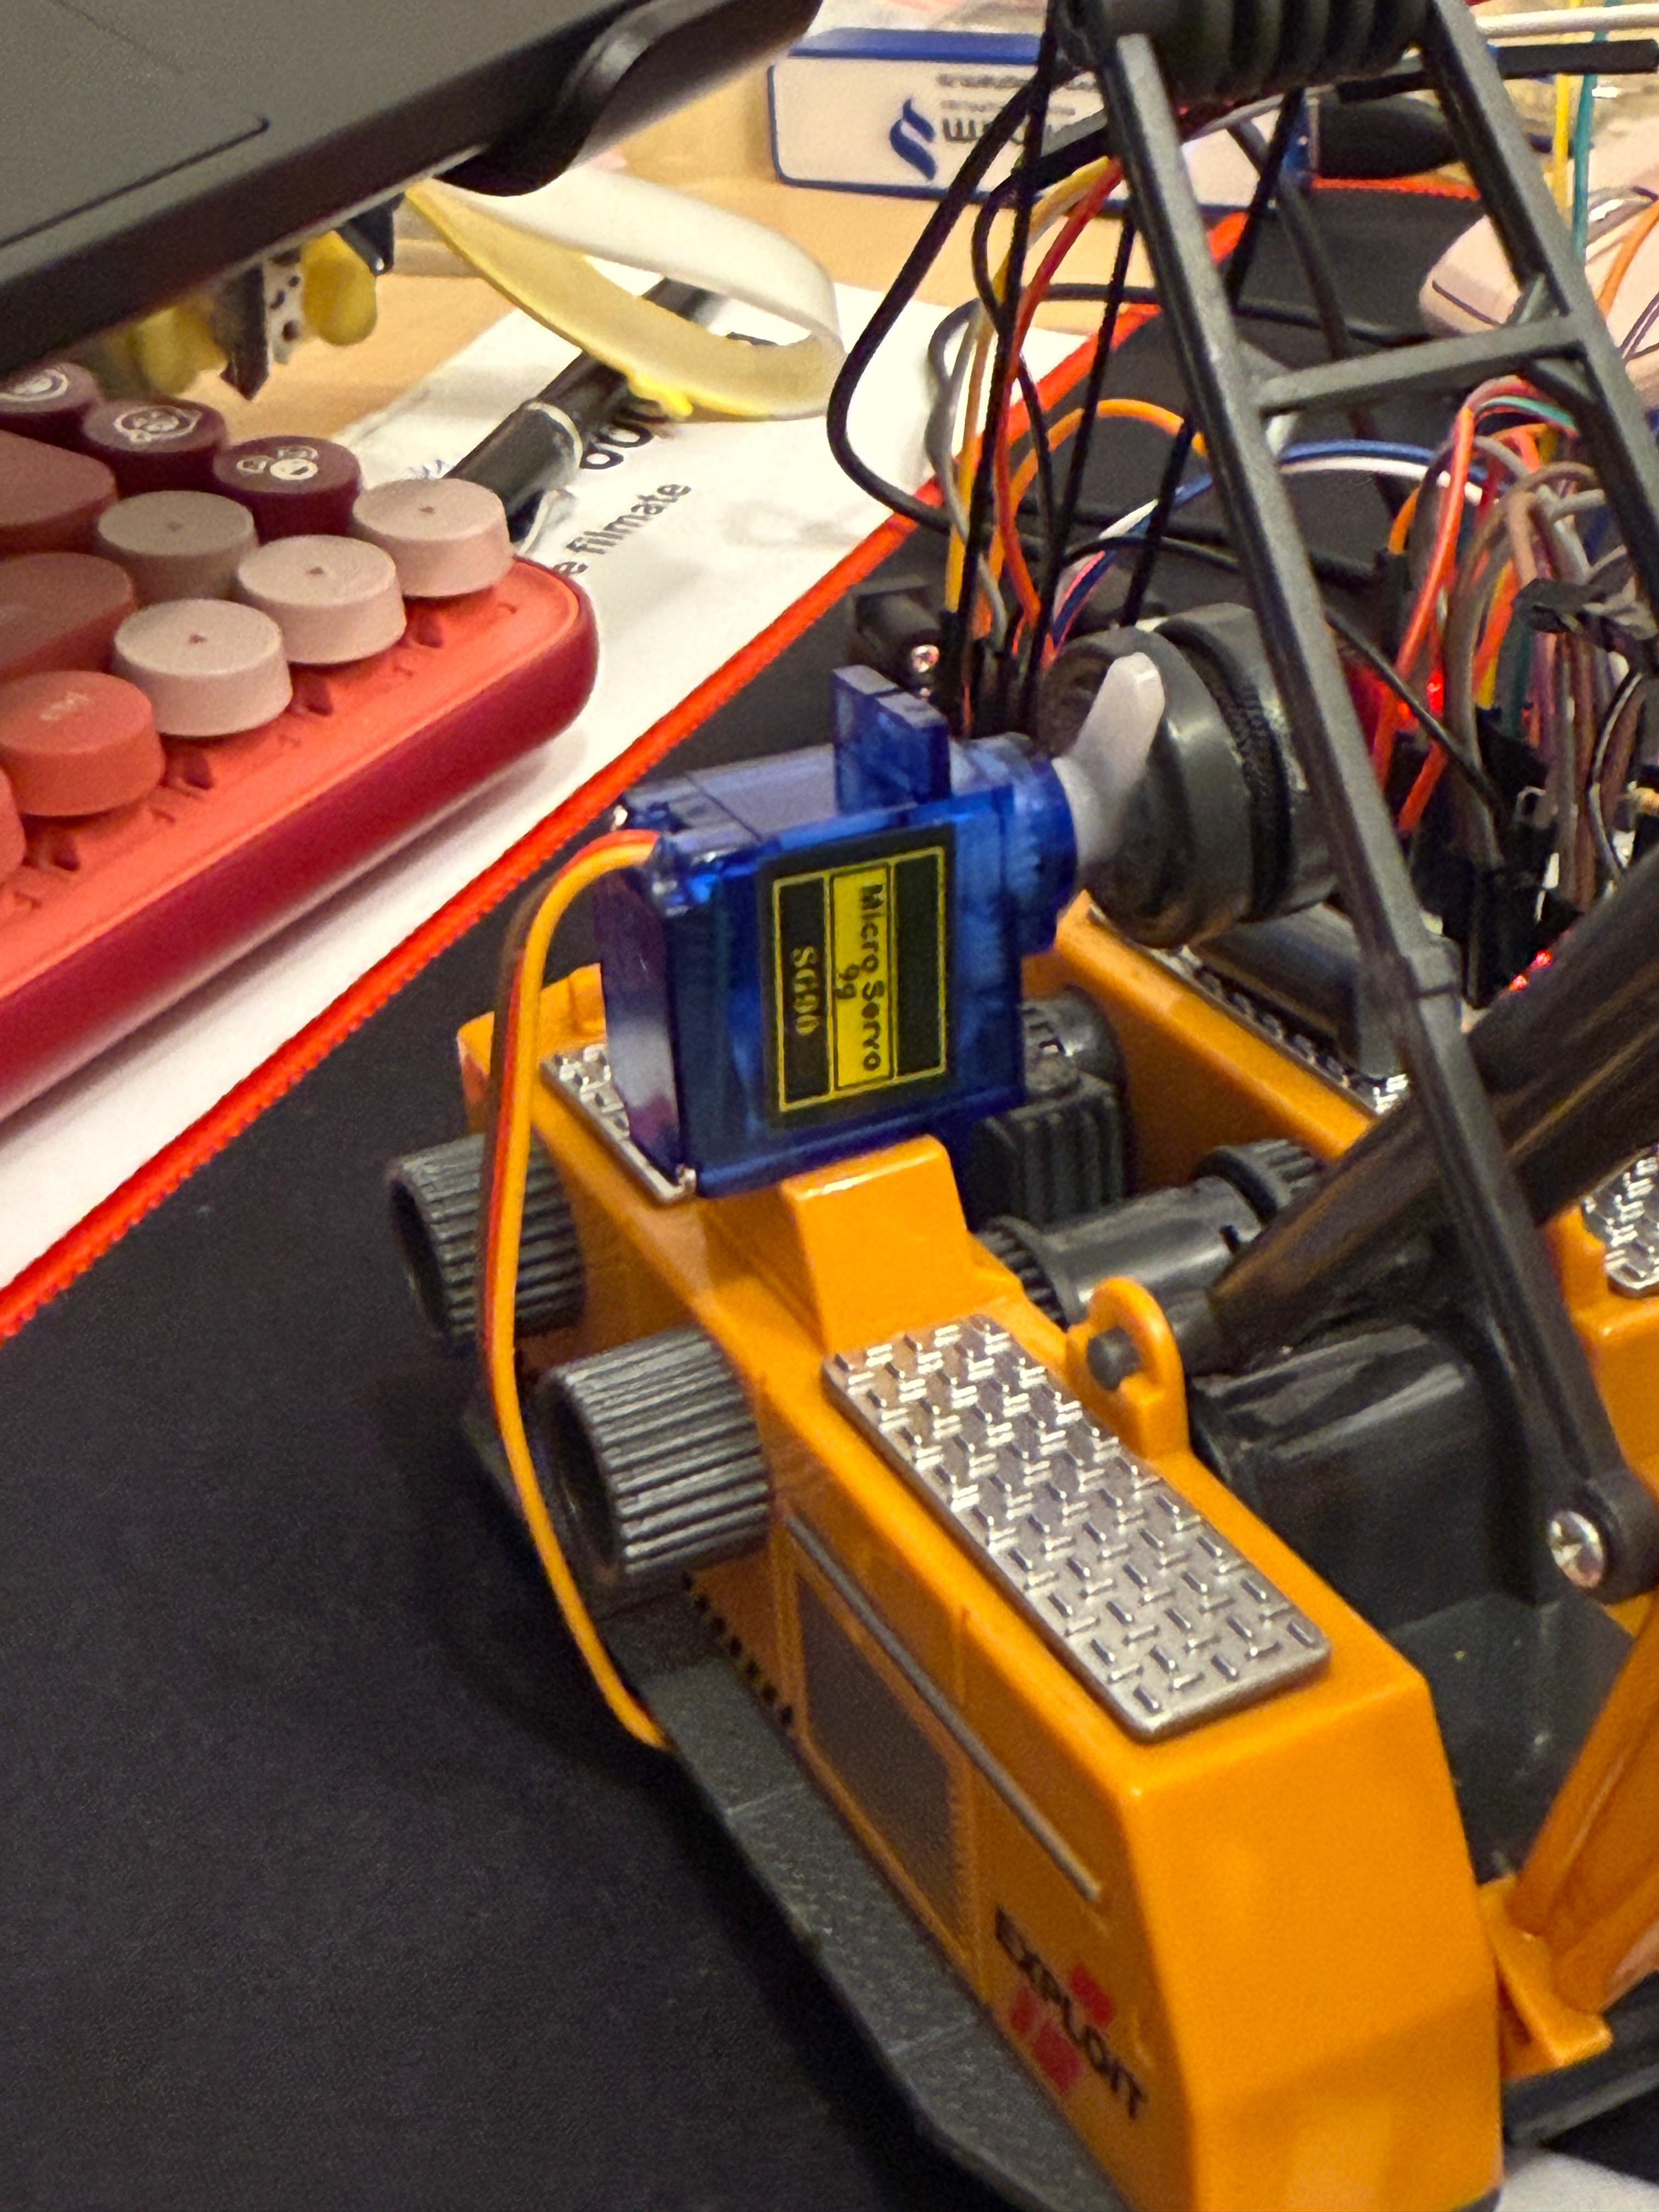
\includegraphics[width=\textwidth]{figures/4.jpg}
      \caption{Servomotor}
  \end{subfigure}
  \hfill
  \begin{subfigure}[b]{0.3\textwidth} % 5-a imagine
      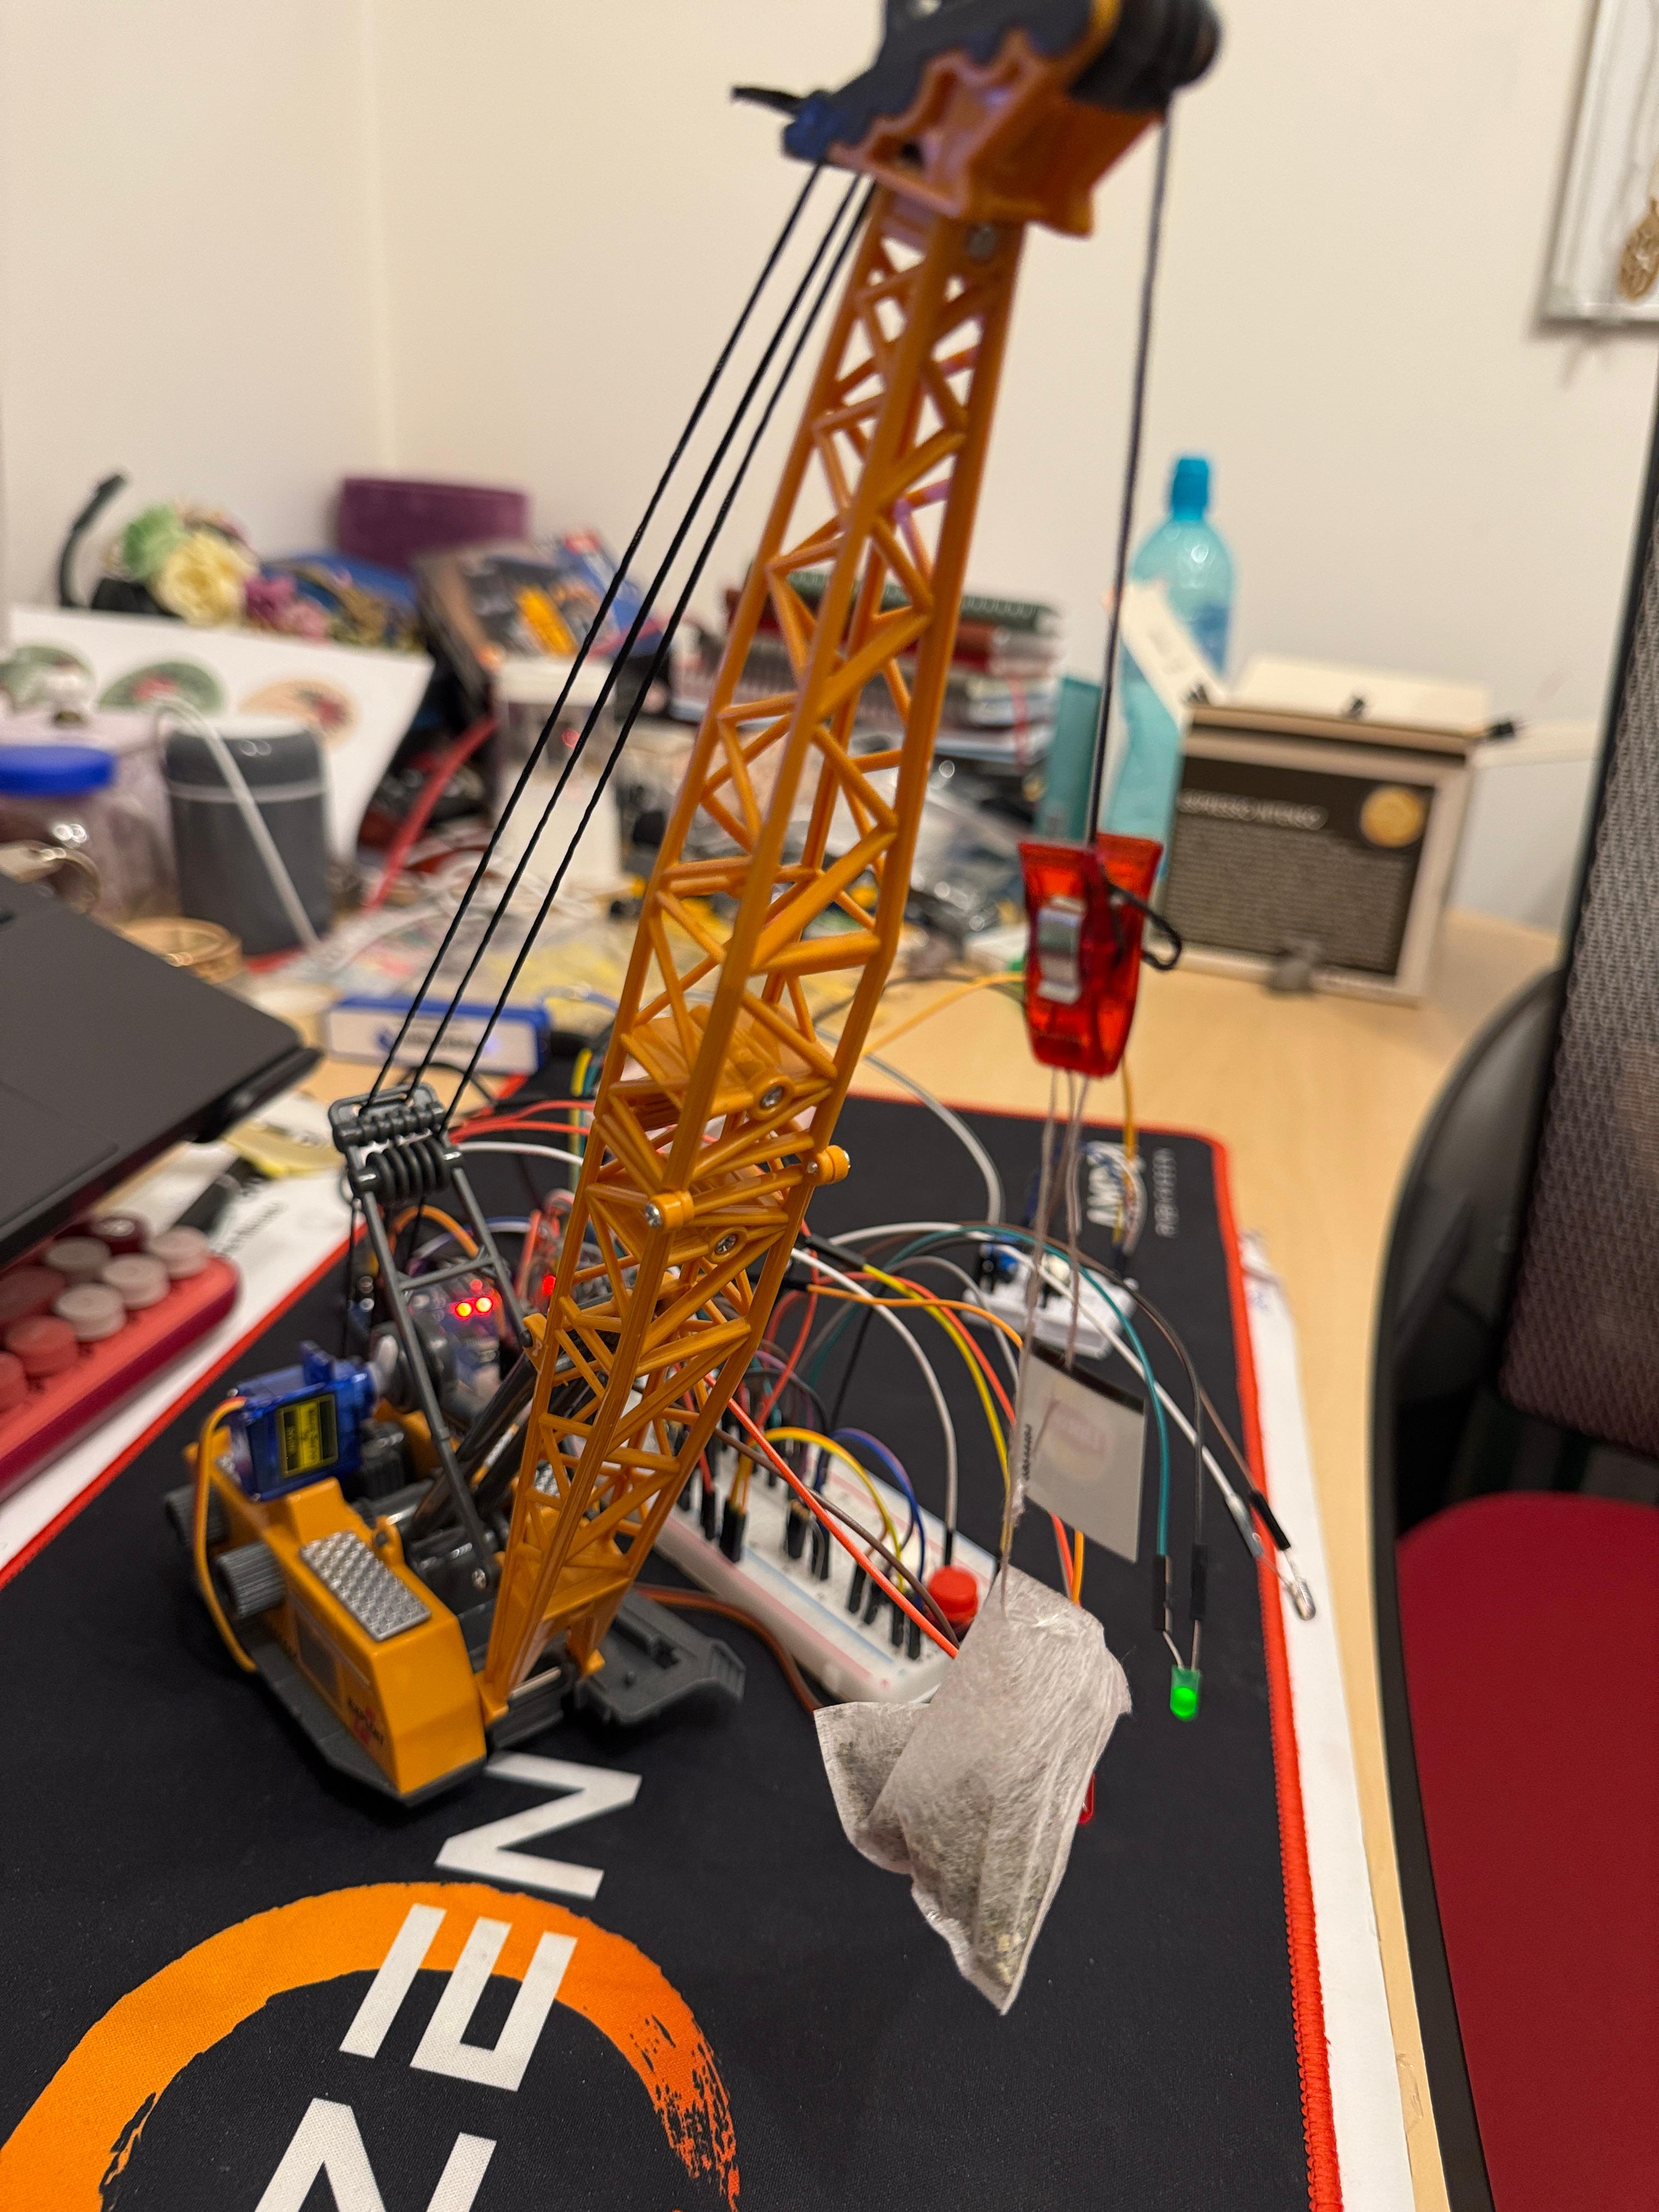
\includegraphics[width=\textwidth]{figures/5.jpg}
      \caption{Macara de jucărie}
  \end{subfigure}

  \caption{Componente și Conexiuni}
  \label{fig:matrice_imagini}
\end{figure}

\begin{figure}[ht!]
  \centering
  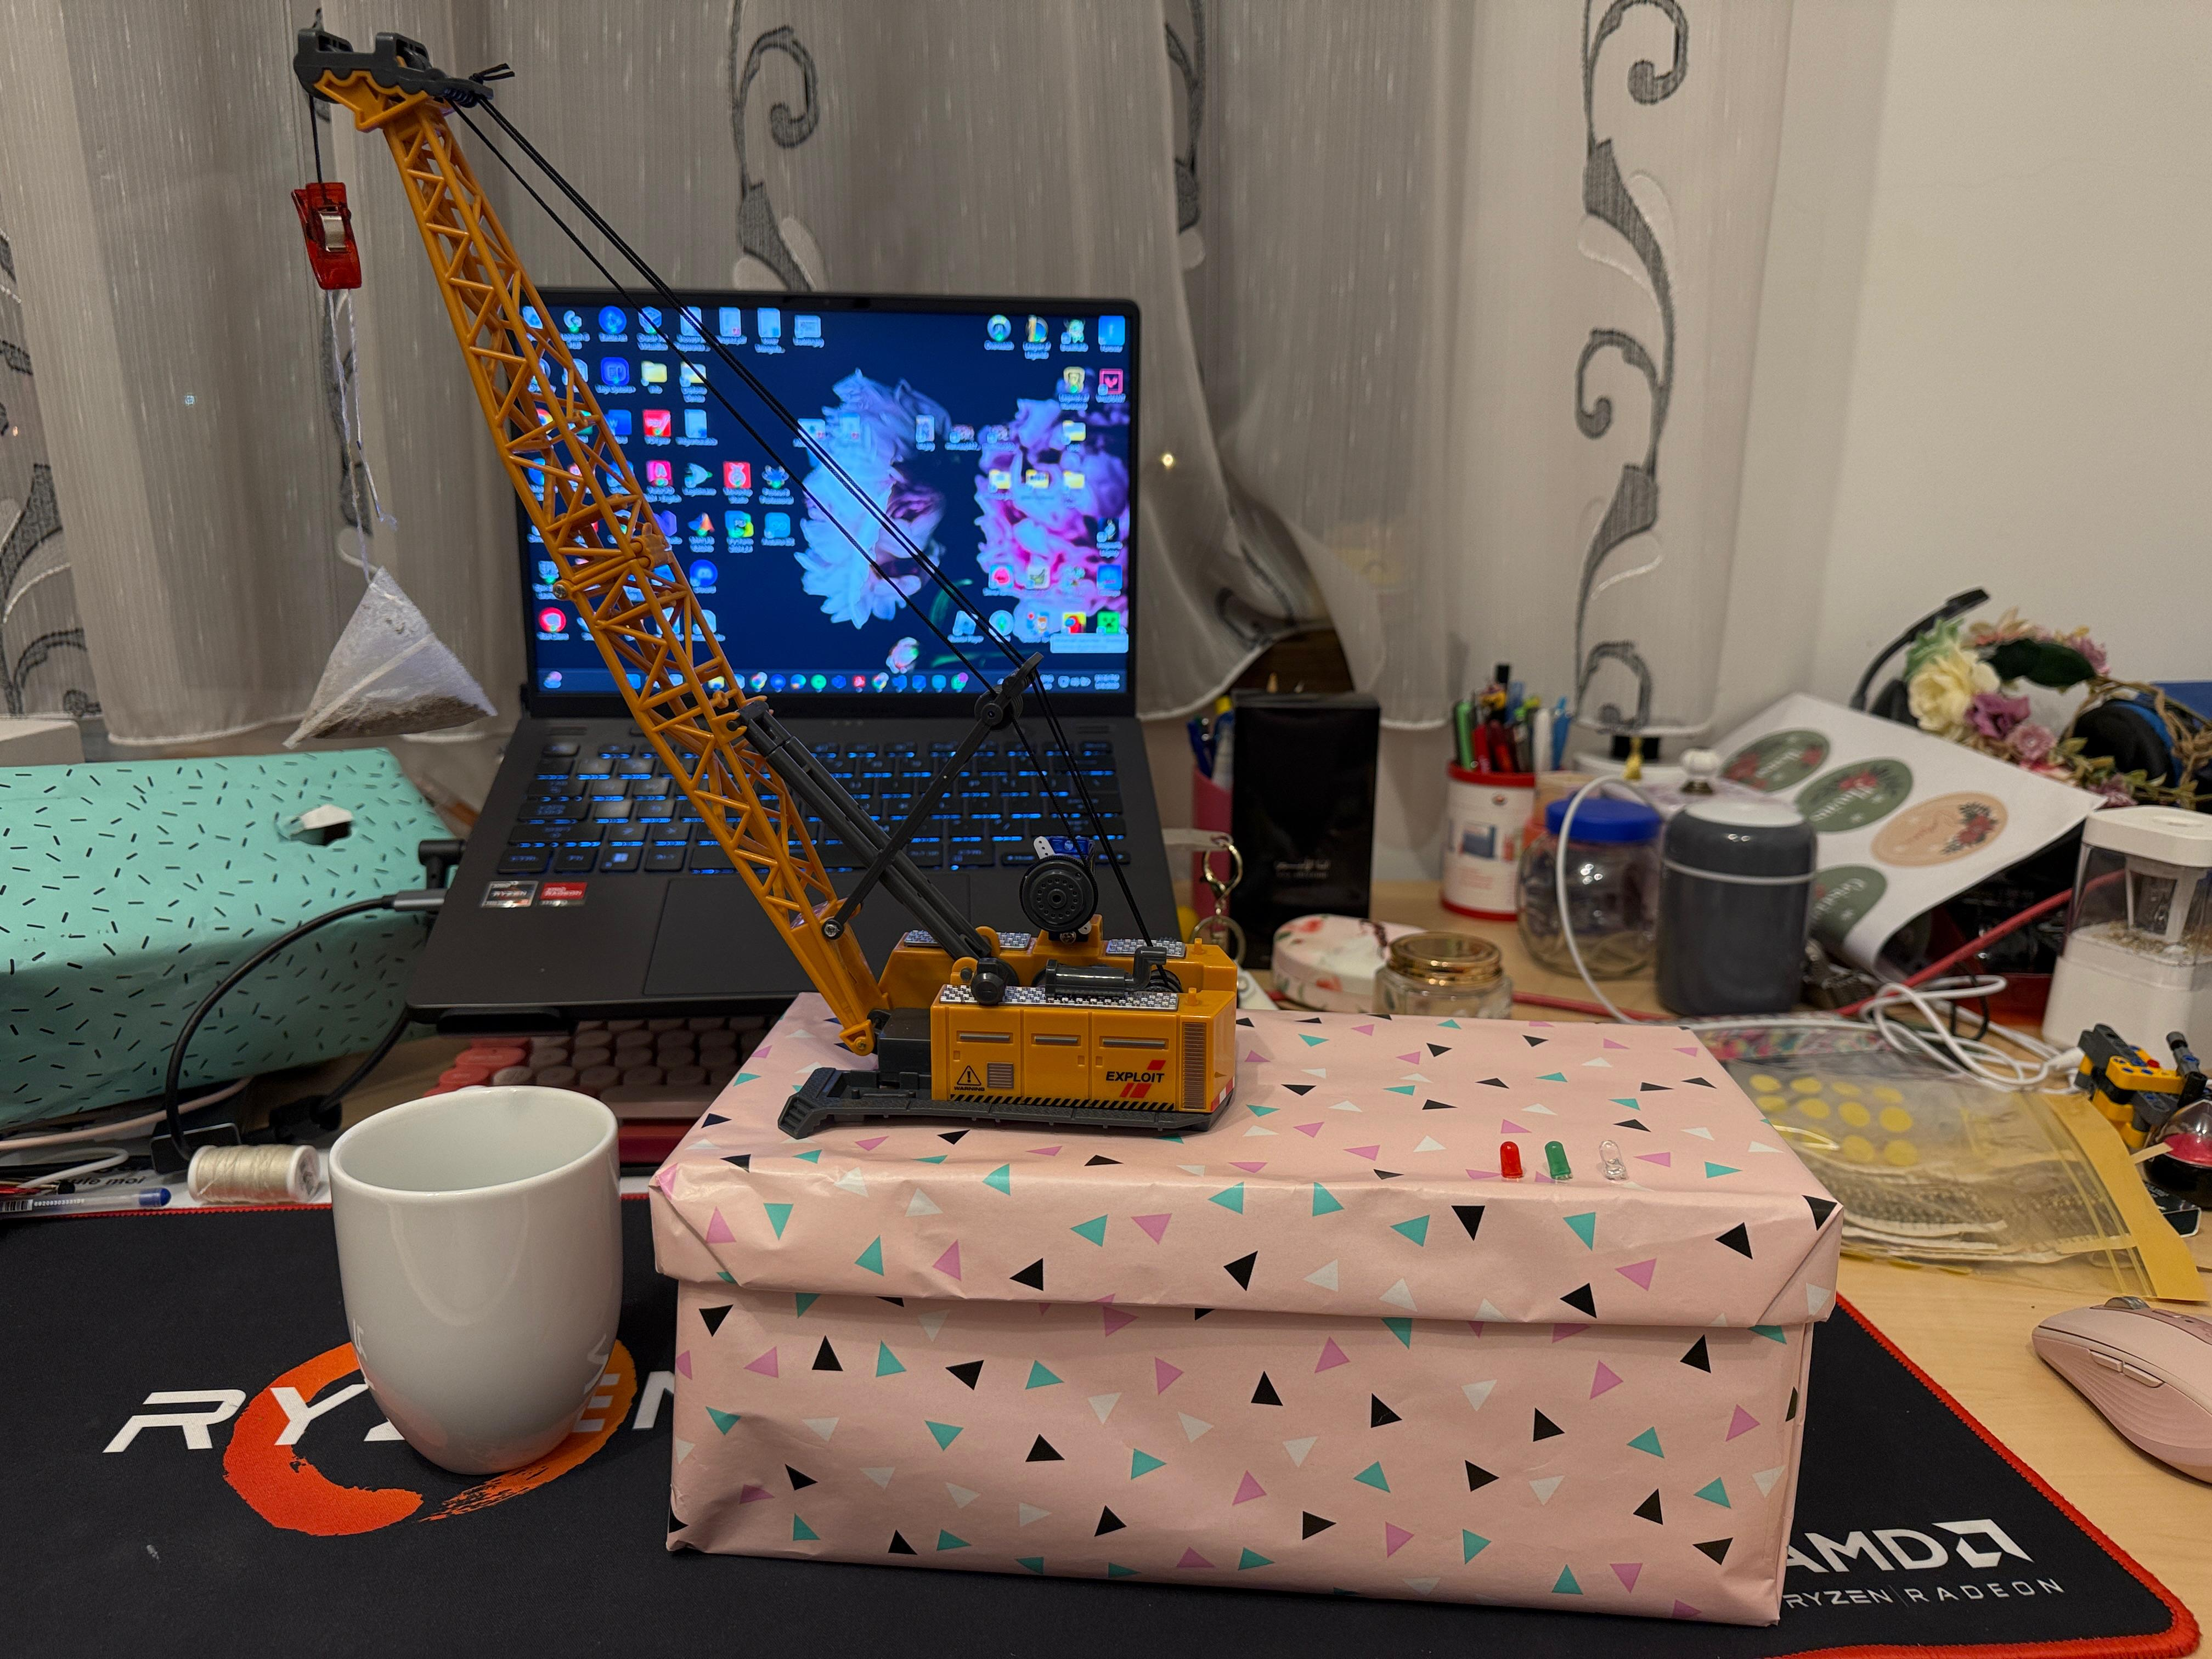
\includegraphics[width=\textwidth]{figures/6.jpg} 
  \caption{Asamblarea Finală}
  \label{fig:fig4}
\end{figure}